\begin{figure}
\begin{minipage}[l]{0.49\textwidth}
	\centering
	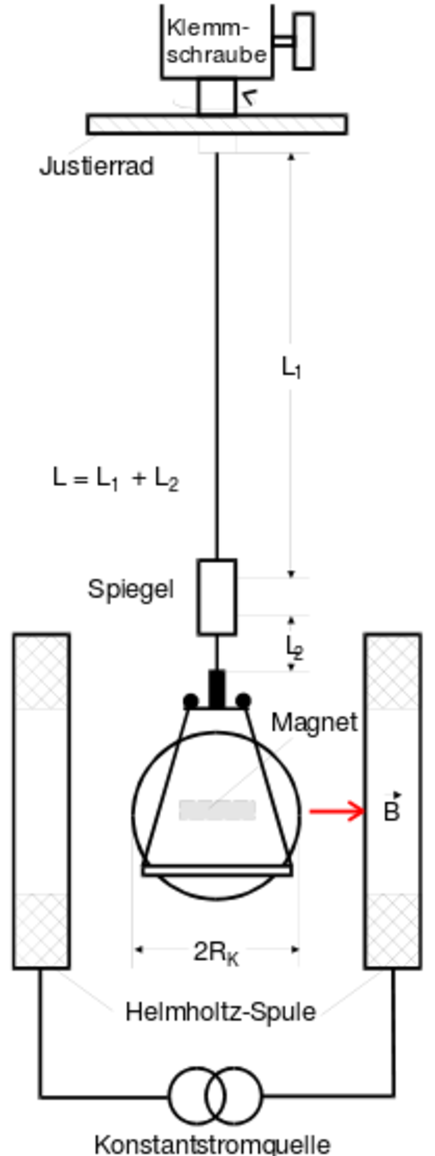
\includegraphics[width=0.4\textwidth]{Bilder/Aufbau1.pdf}
	\caption{Aufbau der Messapparatur. \cite{V102}}
	\label{fig:aufbau1}
\end{minipage}
\begin{minipage}[r]{0.49\textwidth}
	
Abbildung \ref{fig:aufbau1} zeigt die Messapparatur. 
Am unteren Ende eines einseitig fest eingespannten Drahtes ist eine Kugel befestigt, in deren Innern sich ein Permanentmagnet befindet. 
Sie hängt zwischen \textsc{Helmholtz}-Spulen, die bei ein annähernd homogenes Magnetfeld erzeugen, sobald sie von einem Strom $I$ durchflossen werden.
In der unteren Drahthälfte wird dieser durch einen kleinen Spiegel unterbrochen, der zur Bestimmung der Periodendauer benötigt wird.
\label{sec:durchfuehrung2}
\end{minipage}
\end{figure}